%\documentclass[a4paper,10pt]{article}
%\documentclass{beamer}
% \documentclass[a4,notes]{seminar}
\documentclass[handout,notheorems,noamsthm]{beamer}

% Beamer already defines lemma, definition, etc. -> use notheorems
% http://www2.informatik.hu-berlin.de/~mischulz/beamer.html

\usepackage[utf8x]{inputenc}
\usepackage{palatino} %Schriftart

%\usepackage{titlesec}
%\usepackage[fleqn]{amsmath}
\usepackage{amsthm}
\usepackage{amstext}
\usepackage{amssymb}
\usepackage{mathtools}
\usepackage{xparse}
\usepackage{url}
\usepackage{cleveref}
\usepackage{mdframed}
\usepackage{tikz}


%!TEX root =  index.tex

% some useful stuff:
% http://www.automata.rwth-aachen.de/material/skripte/latex/latex.pdf
% http://en.wikibooks.org/wiki/LaTeX/Mathematics
% http://en.wikibooks.org/wiki/LaTeX/Advanced_Mathematics
% http://en.wikibooks.org/wiki/LaTeX/Theorems

\newtheorem{thm}{Theorem}[section]
\newtheorem{lem}[thm]{Lemma}

\theoremstyle{definition}\newtheorem{mydef}{Definition}[section]
\theoremstyle{plain}\newtheorem{lemma}{Lemma}[section]
\theoremstyle{definition}\newtheorem{algo}{Algorithm}[section]

\newcommand{\K}{\mathcal{K}}
\newcommand{\Reg}{\text{Reg}}
\newcommand{\Lang}{\mathcal{L}}
\newcommand{\A}{\mathcal{A}}
\newcommand{\T}{\mathcal{T}}
\newcommand{\F}{\mathcal{F}}
\newcommand{\Q}{\mathbb{Q}}
\newcommand{\R}{\mathbb{R}}
\newcommand{\N}{\mathbb{N}}
\newcommand{\B}{\mathbb{B}}
\newcommand{\Power}{\mathcal{P}}

\newcommand{\mathtext}[1]{\textup{\textrm{#1}}}
\newcommand{\PT}{\mathtext{PT}}
\newcommand{\LT}{\mathtext{LT}}

% got some help here: http://tex.stackexchange.com/questions/13554/define-something-like-lim-but-for-another-name

\newcommand{\ext}{\operatorname{ext}}
\newcommand{\Inf}{\operatorname{Inf}}
\newcommand{\BC}{\operatorname{BC}}
\newcommand{\dext}{\operatorname{\overline{ext}}}
\newcommand{\dlim}{\operatorname{\overline{lim}}}
\newcommand{\Kleene}{\operatorname{\widehat{Kleene}}}
\newcommand{\limClosure}{\operatorname{\widehat{lim}}}
\newcommand{\Occ}{\operatorname{Occ}}
\newcommand{\existsinf}{\exists^\omega}
\newcommand{\overx}{\overset{\times}}
%\newcommand{\overx}{\stackrel{\times}}
\newcommand{\Ax}{\overx{\A}}
\newcommand{\Langreg}{\Lang^*(\text{reg})}
\newcommand{\LangOreg}{\Lang^\omega(\text{reg})}

\newcommand{\defword}[1]{{\bf #1}}

% inspired by http://ftp.fernuni-hagen.de/ftp-dir/pub/mirrors/www.ctan.org/macros/latex/contrib/braket/braket.sty
\def\mid@vertical{\mskip1mu\vrule\mskip1mu}
\def\midvert{\egroup\;\mid@vertical\;\bgroup}
\NewDocumentCommand\Set{mg}{%
    \IfNoValueTF{#2}{%
        \ensuremath{\left\{ #1 \right\}}%
    }{%
        \ensuremath{\left\{ {#1} \;\mid@vertical\; {#2} \right\}}%
    }%
}

%\newcommand{\SetS}[1]{\bigl\{ #1 \bigr\}}
%\newcommand{\SetC}[2]{\bigl\{ #1 \bigm| #2 \bigr\}}
%\DeclarePairedDelimiterX\SetC[2]{\lbrace}{\rbrace}{ #1 \,\delimsize|\, #2 }

%\newcommand{\abs}[1]{\mathopen| #1 \mathclose|}
%\newcommand{\Abs}[1]{\left| #1 \right|}
\newcommand{\abs}[1]{\left| #1 \right|}

% http://de.wikibooks.org/wiki/LaTeX-W%C3%B6rterbuch:_today
\def\monthgerman{\ifcase\month \or
  Januar\or Februar\or M\"arz\or April\or Mai\or Juni\or
  Juli\or August\or September\or Oktober\or November\or Dezember\fi}
\def\todaygerman{\number\day.~\monthgerman\space\number\year}


% for PDF
\subject{a structure theory for Omega-languages}
%\keywords{Omega, language}

\title[Kurzform]{Language Operations and a Structure Theory of $\omega$-Languages}
%\subtitle[Kurzform]{Untertitel}
%\author[A. Zeyer]{Albert Zeyer}
%\institute[i7 RWTH]{Lehrstuhl für Informatik 7}
\date{\today}
%\logo{\pgfimage[width=2cm,height=2cm]{hulogo}}
%\titlegraphic{\includegraphics[width=2cm,height=2cm]{hulogo}}

 
\begin{document}

\frame{\titlepage}

%\frame{
%	\frametitle{Inhaltsverzeichnis}
%	\tableofcontents
%	[pausesections]
%}

\begin{frame}[<+->]{Introduction}
\begin{itemize}
\item consider regular $*$-languages

\item look at $\Lang^* \rightarrow \Lang^\omega$ language operators like lim, ext, BC of them, etc.
\begin{enumerate}
\item $\ext(L) := \Set{\alpha \in \Sigma^\omega}{ \exists n \colon \alpha[0,n] \in L} = L \cdot \Sigma^\omega$
\item $\overline{\ext}(L) := \Set{\alpha \in \Sigma^\omega}{ \forall n \colon \alpha[0,n] \in L} = L \cdot \Sigma^\omega$
\item $\lim(L) := \Set{ \alpha \in \Sigma^\omega }{ \forall N \colon \exists n > N \colon \alpha[0,n] \in L } = \Set{ \alpha \in \Sigma^\omega }{ \exists^\omega n \colon \alpha[0,n] \in L }$
\item $\overline{\lim}(L) := \Set{ \alpha \in \Sigma^\omega }{ \exists N \colon \forall n > N \colon \alpha[0,n] \in L }$
\item Kleene-Closure of $\K$: $\bigcup_{i=1}^n U_i \cdot V_i^\omega$, $U_i, V_i \in \K$
\end{enumerate}

\item compare the resulting $\omega$-languages
\end{itemize}
\end{frame}

\begin{frame}{Diagram}
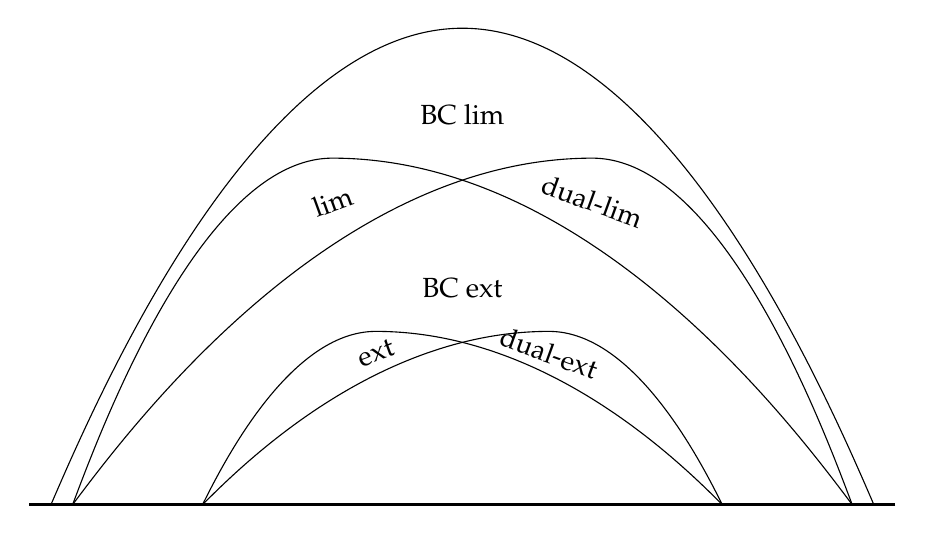
\begin{tikzpicture}
\pgftransformscale{.55}

% http://www.texample.net/tikz/examples/complexity-classes/

%%% HELP LINES - uncomment to design/extend
% \draw[step=1cm,gray,very thin] (-10,0) grid (10,12);
% \node at (0,0) {\textbf{(0,0)}};

%% Horizontal bar
\draw[very thick] (10,0) -- (-10,0);

% BC lim
\draw (-9.5,0) parabola bend (0,11) (9.5,0);
\node at (0,9) {BC lim};

% lim
\draw (-9,0) parabola bend (-3,8) (9,0);
\node[rotate=20] at (-3,7) {lim};

% dual-lim
\draw (-9,0) parabola bend (3,8) (9,0);
\node[rotate=-20] at (3,7) {dual-lim};

% BC ext
%\draw (-6.5,0) parabola bend (0,6) (6.5,0);
\node at (0,5) {BC ext};

% ext
\draw (-6,0) parabola bend (-2,4) (6,0);
\node[rotate=20] at (-2,3.5) {ext};

% dual-ext
\draw (-6,0) parabola bend (2,4) (6,0);
\node[rotate=-20] at (2,3.5) {dual-ext};

\end{tikzpicture}

\end{frame}

\begin{frame}[<+->]{Questions}
\begin{itemize}
\item instead of regular $*$-languages, look at other $*$-language classes, e.g. FO$[<]$ (starfree), FO[+1], \PT, positive \PT, ...
\item does it result in the same relations as in the diagram? are the enclosures strict?
\end{itemize}
\end{frame}

\begin{frame}[<+->]{Some results}
\begin{enumerate}
\item $ \BC \ext \Lang^* (\PT) = \BC \lim \Lang^* (\PT) $
\item $ \Lang^\omega (\mathrm{FO[+1]}) = \BC \ext \Lang^*(\mathrm{FO[+1]}) $
\item $ \Lang^\omega (\mathrm{FO[<]}) = \BC \lim \Lang^*(\mathrm{FO[<]}) $
\item $ \BC \ext \Lang^*( \mathrm{FO[<]} ) \subsetneqq \BC \lim \Lang^* ( \mathrm{FO[<]} )  $
\item $ \BC \ext \Lang^* (\LT) \subsetneqq \BC \lim \Lang^*(\LT) $
\item $ \BC \ext \Lang^* (\mathtext{pos-PT}) = \BC \lim \Lang^* (\mathtext{pos-PT}) $
\item $ \BC \ext \Lang^*(\mathtext{pos-PT}) = \BC \ext \Lang^* (\mathtext{PT}) $
\end{enumerate}
\end{frame}

\begin{frame}[<+->]{More general results}
\begin{enumerate}
\item
$\forall L \in \Lang \colon L \cdot \Sigma^* \in \Lang \linebreak
\Rightarrow \ext(\Lang^*) \subset \lim(\Lang^*)$

\item
$\exists \tilde{L} \in \lim \Lang, \tilde{L} \neq \Sigma^\omega, \forall n \colon \tilde{L}[0,n] = \Sigma^n \linebreak
\Rightarrow \tilde{L} \notin \BC \ext (\Lang) \linebreak
\Rightarrow \BC \ext (\Lang) \neq \BC \lim (\Lang)$

\end{enumerate}
\end{frame}

\end{document}
